\section{Experiments}
\label{sec:experiments}

\subsection{Setup}
\label{sec:setup}

\paragraph{Data and protocol.}
Validation and test labels are hidden, so we hold out 2 images per class from the training split (20,000 images, fixed seed).
We use this holdout for model selection and ablations, and train on the remaining 43 images per class.
Final models are retrained on all 45 images per class.
Validation and test images are used only to produce submission files.
CodaBench reports top-1 accuracy.
Because the validation set is balanced (5 images per class), top-1 accuracy equals the average per-class accuracy.
Our holdout tracks the server closely: 72.31\% \vs 72.57\% for full fine-tuning and 71.98\% \vs 71.90\% for LoRA.
Differences below about 0.3 points are within holdout noise.
All runs use one seed.

\paragraph{Metrics.}
Latency is the mean time of 100 forward passes of a random $224 \times 224$ input at batch size 1, after 10 warm-up passes, with bf16 autocast on an A100.
Throughput is measured at batch size 256.
Repeated measurements of the same architecture vary by about $\pm$0.4\,ms.
GPU-hours are taken from the clock described in \cref{sec:budget}.
Peak VRAM is the maximum memory allocated by PyTorch during training; the memory reserved by PyTorch is 0.2--1.4\,GB higher (20.1\,GB for the final model).
The appendix contains the supporting material:
\begin{itemize}[leftmargin=*,itemsep=0pt,topsep=2pt]
    \item training-log excerpts with time and VRAM (\cref{sec:logs});
    \item all 17 runs (\cref{tab:all-runs});
    \item the full hyperparameters (\cref{tab:hparams}).
\end{itemize}

\paragraph{Hardware and software.}
All runs use one NVIDIA A100-SXM4-80GB with 12 CPU cores, except one ablation batch (random and prototype heads for LoRA in \cref{tab:head}), which ran on an RTX PRO 6000 Blackwell.
Repeating its prototype run on the A100 gave 71.98\% \vs 72.00\%, so accuracies are comparable across the two GPUs; speeds and latencies are not.
Software, as logged for our last two batches, which include all final models: PyTorch 2.11.0 (CUDA 13.0), timm 1.0.30 and PEFT 0.21.1. Earlier runs used the then-current releases, which were not logged.

\subsection{Reproducing the reference baselines}

\begin{table}[t]
  \centering
  \footnotesize
  \setlength{\tabcolsep}{4pt}
  \begin{tabular}{@{}lccc@{}}
    \toprule
    Method & Trainable & Reference & Ours \\
    \midrule
    Zero-shot, initialized head & 0\% & 43.7 & 43.95 \\
    Full fine-tuning & 100\% & 70.8 & 70.88 \\
    LoRA ($r=8$) & 0.34\% & 68.3 & 68.57 \\
    \bottomrule
  \end{tabular}
  \caption{\textbf{Reproducing the reference results} from the project description (top-1, \%).
  Ours: holdout accuracy of 3-epoch runs (0.40--0.45 GPU-h) with the linear-probe head; for zero-shot, the prototype head without training.}
  \label{tab:baselines}
\end{table}

Before changing anything, we checked our pipeline against the three reference results in the project description.
Short 3-epoch runs reproduce all three within 0.3 points (\cref{tab:baselines}).
This confirms the data pipeline, the evaluation and our reading of the trainable-parameter convention.

\subsection{Main results}
\label{sec:main}

\begin{table*}[t]
  \centering
  \footnotesize
  \setlength{\tabcolsep}{4pt}
  \begin{tabular}{@{}llcrrrrrrrrr@{}}
    \toprule
    & & & \multicolumn{2}{c}{Trainable params} & \multicolumn{3}{c}{Top-1 accuracy (\%)} & \multicolumn{2}{c}{Inference} & \multicolumn{2}{c}{Training} \\
    \cmidrule(lr){4-5} \cmidrule(lr){6-8} \cmidrule(lr){9-10} \cmidrule(l){11-12}
    Method & Head init & Ep. & Backbone & Head & Holdout & Val & Test & ms (bs 1) & img/s & GPU-h & GB \\
    \midrule
    Zero-shot & prototype & 0 & 0 & 0 & 43.95 & -- & -- & 7.55 & 3,832 & 0.11 & 3.9 \\
    Linear probe & LP & -- & 0 & 7.69M & 62.07 & -- & -- & -- & -- & $\approx$0.11 & -- \\
    \midrule
    Full fine-tuning & LP & 8 & 85.80M (100\%) & 7.69M & 72.31 & 72.57 & -- & 7.35 & 3,864 & 1.03 & 18.9 \\
    \textbf{Full fine-tuning (final)}$^\dagger$ & prototype & 8 & 85.80M (100\%) & 7.69M & -- & \textbf{76.22} & \todo{TBD} & 14.95$^\ddagger$ & 1,919$^\ddagger$ & 1.03 & 18.9 \\
    \midrule
    LoRA, qkv only & LP & 3 & 0.29M (0.344\%) & 7.69M & 68.57 & -- & -- & 7.22 & 3,817 & 0.40 & 13.5 \\
    AdaptFormer & LP & 3 & 1.19M (1.387\%) & 7.69M & 69.05 & -- & -- & 9.89 & 3,461 & 0.39 & 12.8 \\
    \textbf{LoRA, all linear (final)} & prototype & 3 & 1.18M (1.375\%) & 7.69M & \textbf{71.98} & \textbf{71.90} & \todo{TBD} & 7.61 & 3,869 & 0.54 & 19.9 \\
    \bottomrule
  \end{tabular}
  \caption{\textbf{Main results.}
  Holdout: 2 images per class held out from the training split; Val/Test: CodaBench validation/test (Phase 2).
  Backbone trainable parameters are also given as a fraction of the 85.8M backbone; the 10,000-way head (7.69M) is trained in every method except zero-shot.
  Latency, throughput, GPU-hours and peak VRAM are measured on one A100-SXM4-80GB; LoRA is evaluated after merging.
  $^\dagger$Trained on all 45 images per class (no holdout). $^\ddagger$With flip TTA (two forward passes); without TTA the architecture is identical to the row above it (7.35\,ms).}
  \label{tab:main}
\end{table*}

\begin{figure}[t]
  \centering
  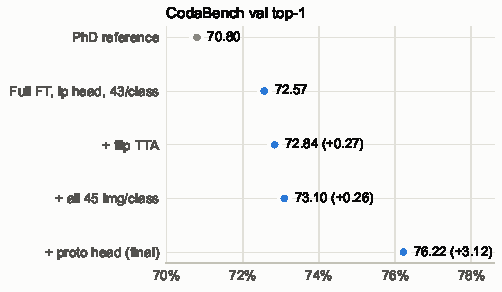
\includegraphics[width=\linewidth]{figures/fig1_codabench_progression_col.pdf}
  \caption{\textbf{CodaBench validation accuracy as we change one setting at a time} (all runs: full fine-tuning, 8 epochs). The gray dot is the reference. Positions encode values, so the axis starts at 70\%.}
  \label{fig:progression}
\end{figure}

\Cref{tab:main} reports all four required metrics for the key models.
Our final full fine-tuning model reaches \textbf{76.22\%} on the CodaBench validation set, 5.4 points above the reference.
It uses 1.03 GPU-hours, 18.9\,GB of memory and the unchanged ViT-B/16 architecture.
\Cref{fig:progression} shows how we got there, one change at a time:
\begin{itemize}[leftmargin=*,itemsep=0pt,topsep=2pt]
    \item flip TTA adds 0.27 points; it changes 4.6\% of the predictions and doubles latency;
    \item training on all 45 images per class adds 0.26 points, which is at the edge of the noise but in the expected direction;
    \item replacing the LP head by the prototype head adds \textbf{3.12 points}.
\end{itemize}
Our final PEFT model, LoRA on all linear layers with a prototype head, reaches \textbf{71.90\%} (+3.6 over the reference LoRA).
It trains 1.375\% of the backbone, and after merging it has exactly the latency of the base model.
Under identical settings (3 epochs, prototype head, holdout), it attains 98\% of full fine-tuning accuracy (71.98\% \vs 73.38\%).
\todo{Phase 2: add CodaBench test accuracy of the final models.}

\subsection{Ablation: classifier head initialization}
\label{sec:ablation-head}

\begin{table}[t]
  \centering
  \footnotesize
  \setlength{\tabcolsep}{4pt}
  \begin{tabular}{@{}lcccc@{}}
    \toprule
    Head init & \shortstack{Head\\alone} & \shortstack{LoRA all\\3 ep\\holdout} & \shortstack{Full FT\\3 ep\\holdout} & \shortstack{Full FT\\8 ep, TTA\\val} \\
    \midrule
    Random & chance & 71.95$^*$ & -- & -- \\
    Prototype & 44.0 & \textbf{72.00}$^*$ & \textbf{73.38} & \textbf{76.22} \\
    Linear probe (LP) & 62.1 & 69.45 & 70.88 & 73.10 \\
    \bottomrule
  \end{tabular}
  \caption{\textbf{Head initialization} (top-1, \%). Within each column only the head initialization changes.
  Head alone: accuracy of the initialized head before training. Full FT 8 ep: all 45 images per class, flip TTA, CodaBench validation.
  $^*$RTX PRO 6000; repeating the prototype run on the A100 gives 71.98.}
  \label{tab:head}
\end{table}

\begin{figure*}[t]
  \centering
  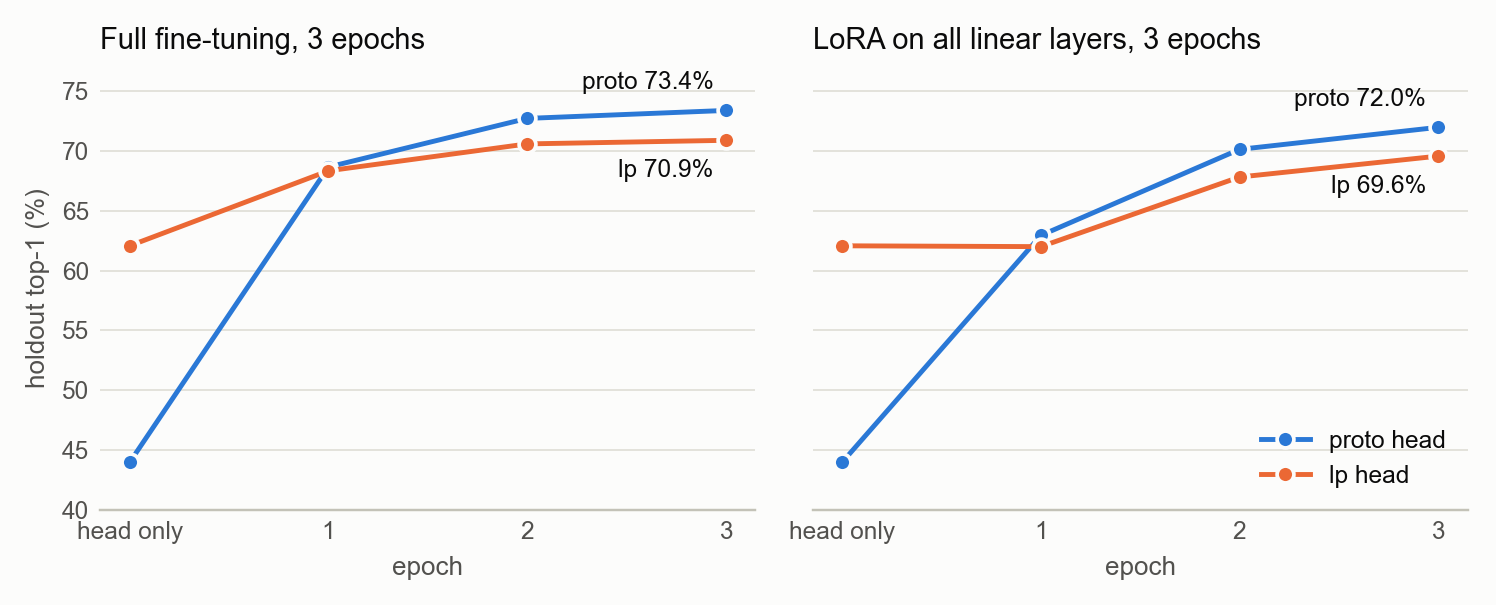
\includegraphics[width=0.92\textwidth]{figures/fig2_head_init_holdout.png}
  \caption{\textbf{Holdout accuracy during training for the LP and prototype heads} (3 epochs; left: full fine-tuning, right: LoRA on all linear layers).
  ``head only'' is the accuracy of the initialized head before any training.
  The LP head starts 18 points higher but finishes about 2.5 points lower.}
  \label{fig:head-curves}
\end{figure*}

\begin{figure*}[t]
  \centering
  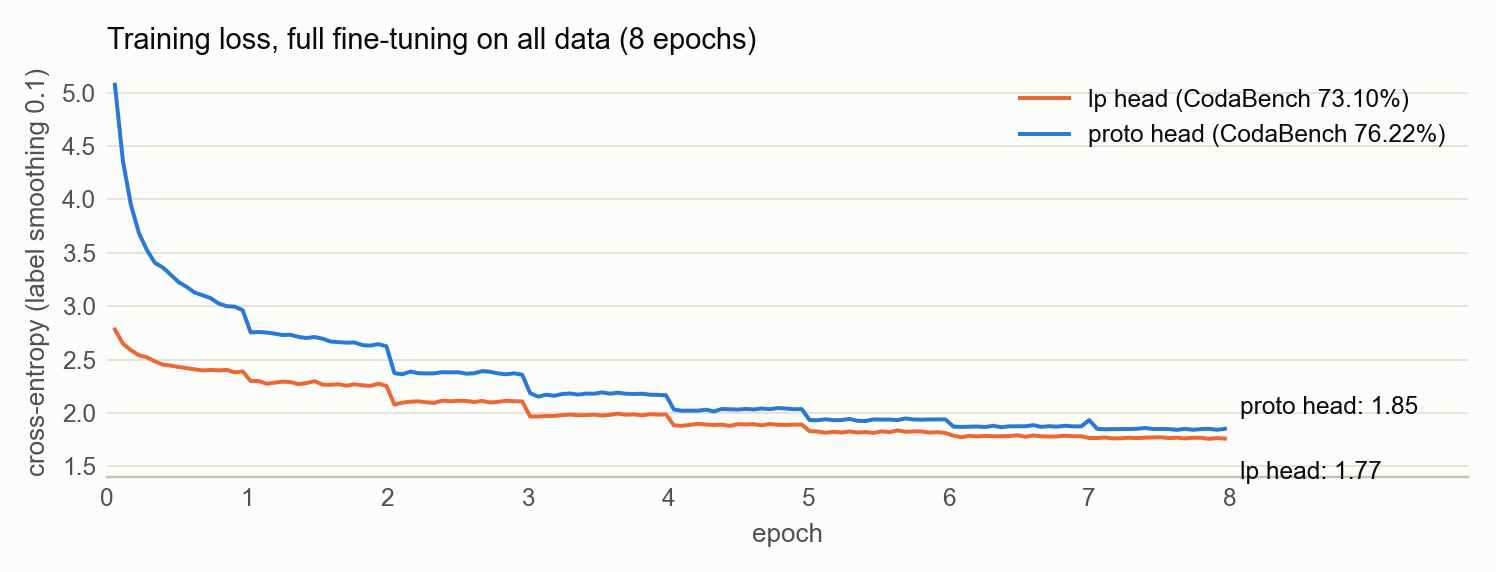
\includegraphics[width=0.92\textwidth]{figures/fig3_loss_lp_vs_proto.png}
  \caption{\textbf{Training loss of full fine-tuning on all data (8 epochs) with the LP and prototype heads}, which differ only in head initialization.
  The prototype model keeps a \emph{higher} training loss (1.85 \vs 1.77 in the last epoch) but scores 3.12 points higher on the validation set.
  The loss drops at every epoch boundary and stays flat within an epoch, a sign that the model is memorizing the 45 images per class.}
  \label{fig:loss}
\end{figure*}

\Cref{tab:head} isolates the head initialization in three settings.
In all three, the LP head is clearly worst, 2.5--3.1 points below the prototype head.
Random and prototype initialization end up level for LoRA (71.95\% \vs 72.00\%).
The prototype head, however, learns faster: it leads by 5 points after the first epoch (63.3\% \vs 58.4\%).
\Cref{fig:head-curves} shows the paradox: the LP head is 18 points better before training and worse after it.

We attribute the LP penalty to the probe having been fitted on \emph{the same images that are then used for fine-tuning}.
The probe already fits them well.
Averaged over the first 100 steps of the LoRA runs, the training loss is 2.29 with the LP head, compared with 4.39 with the prototype head and 9.28 with a random head.
The fine-tuning gradient reaching the backbone is therefore small and dominated by the few examples the probe gets wrong.
Once the features start to move, the fitted head no longer matches them: in the LoRA run with the LP head, the training loss \emph{rises} from 2.22 to 2.69 during the first epoch, before any image has been seen twice.
\Cref{fig:loss} points the same way.
With identical full fine-tuning settings, the LP model reaches a lower training loss but a much lower validation accuracy, \ie, it memorizes more and generalizes less.
A prototype head encodes the class structure, which explains its faster start, without having been fitted to individual training images.
This complements LP-FT~\cite{kumar2022lpft}, which motivates the probe as protection against feature distortion: when the probe is fitted on the fine-tuning images themselves, with only 43--45 images per class, it becomes a liability.

\subsection{Ablation: where to put PEFT capacity}
\label{sec:ablation-peft}

\begin{table}[t]
  \centering
  \footnotesize
  \setlength{\tabcolsep}{3pt}
  \begin{tabular}{@{}lrrrrr@{}}
    \toprule
    LP head, 3 epochs & Params & Holdout & img/s & GB & ms \\
    \midrule
    LoRA qkv, lr $10^{-3}$ & 0.344\% & 68.57 & 1,341 & 13.5 & 7.22 \\
    LoRA qkv, lr $5{\times}10^{-4}$ & 0.344\% & 68.45 & 1,353 & 13.5 & 7.15 \\
    LoRA all linear & 1.375\% & \textbf{69.45} & 885 & 19.9 & 7.03 \\
    AdaptFormer & 1.387\% & 69.05 & 1,437 & 12.8 & 9.89 \\
    \midrule
    Full fine-tuning & 100\% & 70.88 & 1,131 & 18.9 & 7.31 \\
    \bottomrule
  \end{tabular}
  \caption{\textbf{PEFT design.} Params: trainable backbone parameters (head excluded). img/s: training throughput; GB: peak training memory; ms: batch-1 latency after merging (A100, bf16).}
  \label{tab:peft}
\end{table}

\Cref{tab:peft} compares PEFT variants with the LP head for 3 epochs.
\textbf{Capacity matters more than the learning rate.}
Halving the LoRA learning rate changes nothing (\minus0.12, within noise).
Extending LoRA from \texttt{qkv} to all four linear layers, so that the MLP is also adapted, adds 0.88 points while staying far below the 5\% budget for trainable parameters.
\textbf{Mergeable updates matter for deployment.}
AdaptFormer is close in accuracy, but its parallel branches cannot be merged and raise batch-1 latency from about 7.3\,ms to 9.89\,ms ($+$35\%).
\textbf{PEFT does not imply cheaper training here.}
LoRA on all linear layers trains \emph{slower} than full fine-tuning (885 \vs 1,131 img/s) and peaks slightly higher in memory (19.9 \vs 18.9\,GB).
This is presumably because of the 96 extra small, unfused matrix multiplications per forward pass and the activations they keep for the backward pass.
Its savings are in trainable parameters, optimizer state and checkpoint size (35.5\,MB, of which 30.8\,MB is the head, \vs 374\,MB).

\subsection{Ablation: training length}
\label{sec:ablation-length}

\begin{table}[t]
  \centering
  \footnotesize
  \setlength{\tabcolsep}{3.5pt}
  \begin{tabular}{@{}lrrr@{}}
    \toprule
    Setting & Short (ep) & Long (ep) & $\Delta$ \\
    \midrule
    Full FT, LP & 70.88 (3) & 72.31 (8) & $+$1.43 \\
    Full FT, prototype, final$^\ddagger$ & 74.01 (3) & 76.22 (8) & $+$2.21 \\
    LoRA qkv, LP$^\dagger$ & 68.57 (3) & 68.69 (10) & $+$0.12 \\
    LoRA all, LP & 69.45 (3) & 69.87 (6) & $+$0.42 \\
    LoRA all, prototype & 71.98 (3) & 71.52 (6) & \minus0.46 \\
    \bottomrule
  \end{tabular}
  \caption{\textbf{Training length} (holdout top-1, \%; LoRA all: LoRA on all linear layers).
  $^\ddagger$All 45 images per class with flip TTA, CodaBench validation.
  $^\dagger$The 10-epoch run also lowered the head learning rate to $2{\times}10^{-4}$.}
  \label{tab:length}
\end{table}

The two adaptation styles spend the budget very differently (\cref{tab:length}).
Full fine-tuning keeps improving with longer schedules: going from 3 to 8 epochs adds 2.21 points for the final recipe.
LoRA, in contrast, saturates after about 3 epochs, and with the prototype head 6 epochs are worse than 3.
A plausible explanation is the learning rate.
Full fine-tuning uses a small learning rate ($10^{-4}$) that is further reduced for early layers, while LoRA uses $10^{-3}$.
With only 43 images per class, the longer high-learning-rate phase mainly increases memorization.
Its training loss falls much further in 6 epochs (1.70) than in 3 (1.95), while holdout accuracy falls too.
Hence our final PEFT model uses 3 epochs (0.54 GPU-hours) and our final full fine-tuning model uses 8 epochs (1.03 GPU-hours), both within the 1.2-hour budget.
